\section{Holographic method}\label{ss:Holography}

The holographic principle, stating the equivalence between gauge theory and gravity theory, is implied by string theory.
One of the most famous duality is the AdS/CFT correspondence conjectured
by \textcite{Maldacena:1997re}, which has been the main focus of research in
high energy theory for two decades.
String theory has extended objects called D-branes that allow two complementary descriptions as a black hole in general relativity and a gauge theory on the world volume.
In the former picture, one finds the AdS geometry in the near horizon region, which turns out to be equivalent to the gauge theory of the latter picture.
The AdS/CFT correspondence crystalizes the equivalence by connecting the type IIB superstring theory on the AdS space with a supersymmetric CFT
living on the boundary of the AdS space.
This is a concrete example of duality where a strongly coupled region of one theory is described by a weakly coupled region of the other theory.
Hence the direct check of this correspondence is far reaching in its nature and remains to be proved.

Apart from the string theory implication, we can take the AdS/CFT correspondence 
as a gauge/gravity duality in its own right simply based on the symmetry argument that the isometry $\SO(2,d)$ of the AdS$_{d+1}$ space agrees with 
the conformal group of CFT$_d$.

In this section, we give a quick review of the AdS/CFT
correspondence. 
This subject is comprehensively covered by a review paper by
\textcite{Aharony:1999ti} and many others in the literature including \textcite{Klebanov:2000me,McGreevy:2009xe} from different points of view.
We then introduce the holographic formula of entanglement entropy proposed by \textcite{Ryu:2006bv,Ryu:2006ef} and discuss the implications.
The reviews on entanglement entropy from the holographic point of view can be found in \textcite{Nishioka:2009un,Takayanagi:2012kg,Rangamani:2016dms}.


\subsection{The AdS geometries}

We briefly sketch several types of the useful coordinates for the AdS geometry that we adopt in the following sections.
Table \ref{tab:AdS_Coord_Summary} is the summary of the relations between the AdS coordinates and the corresponding conformally flat spaces on their boundaries.

To begin with, consider the flat $(d+2)$-dimensional pseudo Euclidean space defined by
\begin{align}\label{PseudEuclid}
 \d s^2&= - \d y_{-1}^2 - \d y_0^2 + \d y_1^2 + \cdots + \d y_d^2 \ .
\end{align}
The AdS$_{d+1}$ space with radius $L$ is an embedding hypersurface
satisfying 
\begin{align}
 -y_{-1}^2 - y_0^2 + y_1^2 + \cdots + y_d^2&= -L^2 \ .
\end{align}
This construction manifests the isometry $\SO(2,d)$ of the AdS$_{d+1}$ space.
Among many coordinates in the AdS space we focus on the typical examples,
the global, Poincar{\'e} and hyperbolic coordinates.


\subsubsection{Global coordinates}
The global coordinates are introduced by the coordinate transformations:
\begin{align}
\begin{aligned}
 y_{-1}&= L\,\cosh\rho\, \sin t \ , \\
 y_0&=L\,\cosh\rho\,\cos t \ , \\
 y_i &= L\,\sinh \rho\, \ e^i \ , \quad (i=1,\dots,d)\ ,
\end{aligned}
\end{align}
where $e^i$ satisfy the relation $\sum_{i=1}^d (e^i)^2=1$ and 
span a $d$-dimensional sphere.
The metric Eq.\,\eqref{PseudEuclid} then becomes
\begin{align}
 \d s^2&= L^2\left[ -\cosh^2\rho\, \d t^2 + \d\rho^2 + \sinh^2\rho\,
 \d\Omega_{d-1}^2 \right] \ .
\end{align}
By the coordinate transformation $r = \sinh\rho$, we find
another form of the global coordinates often used in literature,
\begin{align}\label{GlobalAdS}
 \d s^2&= L^2\left[ -\left( r^2+1\right) \d t^2 + \frac{\d r^2}{r^2 + 1
 } + r^2 \,\d\Omega_{d-1}^2 \right]\ .
\end{align}
These coordinates cover the whole AdS$_{d+1}$ space whose boundary at $r=\infty$ is $\BR \times \BS^{d-1}$ space.

The global AdS$_{d+1}$ space can have de Sitter space (dS$_{d}$) as its boundary,
\begin{align}
\d s^2 = L^2 \left[ \d\rho^2 + \sinh^2\rho \left( -\sin^2\theta\, \d t^2 + \d\theta^2 + \cos^2\theta \,\d\Omega_{d-2}^2 \right)\right] \ ,
\end{align}
which follows from the coordinate transformations
\begin{align}
\begin{aligned}
y_{-1} &= L\,\cosh\rho \ , \\
y_0 &= L\,\sinh\rho\, \sin\theta\, \sinh t \ , \\
y_d &= L\,\sinh\rho\, \sin\theta\, \cosh t \ , \\
y_i &= L\,\sinh \rho\, \cos\theta\,  \tilde e^i \ , \qquad (i=1,\cdots, d-1) \ , 
\end{aligned}
\end{align}
where $\sum_{i=1}^{d-1}(\tilde e^i)^2 = 1$.
This is also useful when we consider a holographic dual of a Euclidean QFT on $\BS^d$ after the Wick rotation.


\subsubsection{Poincar{\'e} coordinates}
The Poincar{\'e} coordinates are introduced by the coordinate transformations:
\begin{align}
\begin{aligned}
y_{-1} &= \frac{1}{2r}\left[ 1 + r^2\left(L^2 -t^2 + \sum_{i=1}^{d-1}x_i^2\right)\right] \ , \\
y_0 &= L \,r\, t\ ,\\
y_d &= \frac{1}{2r}\left[ 1 + r^2\left(-L^2 -t^2 + \sum_{i=1}^{d-1}x_i^2\right)\right]  \ , \\
y_i &= L\, r\, x_i\ , \qquad (i=1,\cdots d-1) \ ,
\end{aligned}
\end{align}
whose metric is given by
\begin{align}
 \d s^2&=L^2\left[ \frac{\d r^2}{r^2} + r^2\left(-\d t^2 + \sum_{i=1}^{d-1} \d x_i^2 \right) \right] \ .
\end{align}
These coordinates cover a half portion of the whole AdS$_{d+1}$ space and the boundary at $r=\infty$ is the Minkowski space $\BR^{d-1,1}$.

Inverting the radial coordinate $z\equiv 1/r$ yields another version of the Poincar{\'e} coordinates,
\begin{align}\label{AdS_Poincare_z}
 \d s^2&= L^2\,\frac{\d z^2 - \d t^2 + \sum_{i=1}^{d-1} \d x_i^2}{z^2} \ .
\end{align}



\subsubsection{Hyperbolic coordinates}
The hyperbolic coordinates of the AdS$_{d+1}$ space are obtained by the coordinate transformations:
\begin{align}
\begin{aligned}
y_{-1} &= L\, r\, \cosh u \ , \\ 
y_0 &= L\,\sqrt{r^2 - 1}\, \sinh t \ , \\
y_d &= L\,\sqrt{r^2 - 1}\, \cosh t \ ,  \\
y_i &= L\,r\,\sinh u \,\tilde e^i \ , \qquad (i=1,\cdots,d-1) \ .
\end{aligned}
\end{align}
The resulting metric becomes
\begin{align}\label{AdS_Hyp}
\begin{aligned}
\d s^2 &=L^2\left[  -\left(r^2 - 1 \right) \d t^2 + \frac{\d r^2}{r^2 - 1}\right.\\ 
	&\qquad \left. + r^2 \left( \d u^2 + \sinh^2 u\, \d\Omega_{d-2}^2\right) \right]\ .
\end{aligned}
\end{align}
These coordinates cover a half portion of the whole AdS$_{d+1}$ space whose boundary at $r=\infty$ is $\BR \times \BH^{d-1}$ space.
While these coordinates are locally equivalent to the other coordinates, there is a coordinate singularity at the event horizon, $r=1$.
In Euclidean signature, the Euclidean time $\tau = - \i\, t$ becomes a circle of period  $\beta = 2\pi$ to avoid the conical singularity at the horizon.
The period is identified with an inverse temperature of the dual CFT.


Table \ref{tab:AdS_Coord_Summary} summarizes the relations of the conformally flat (Euclidean) spaces to the corresponding (Lorentzian) AdS metrics.
\begin{table}[htbp]
\caption{\label{tab:AdS_Coord_Summary}Conformally flat spaces and the corresponding Lorentzian AdS metrics.}
\begin{ruledtabular}
\begin{tabular}{llll}
\multicolumn{2}{c}{ Conformally flat space} & \multicolumn{2}{c}{AdS metric}\\ \hline
 $\BR^d$ & Eq.\,\eqref{CFT_Flat} & Poincar{\'e} coordinates & Eq.\,\eqref{AdS_Poincare_z} \\
 $\BS^1 \times \BH^{d-1}$ & Eq.\,\eqref{CFT_Hyp} & Hyperbolic coordinates & Eq.\,\eqref{AdS_Hyp} \\
 $\BS^d$ & Eq.\,\eqref{CFT_Sphere} & Global coordinates & Eq.\,\eqref{GlobalAdS}
\end{tabular}
\end{ruledtabular}
\end{table}




\subsection{The GKP-W relation}
In what follows we deal with the Euclidean case.
The Euclidean AdS$_{d+1}$ spacetime is a solution to the Einstein equation of the Einstein-Hilbert action
\begin{align}\label{EH_action}
\begin{aligned}
I_\text{bulk} [\CB] &= - \frac{1}{16\pi G_N} \int_{\CB} \d^{d+1} x \, \sqrt{g}\, \left(\CR + \frac{d(d-1)}{L^2} \right) \\
	&\qquad - \frac{1}{8\pi G_N} \int_{\partial\CB} \d^d x\, \sqrt{h}\, \CK\ ,
\end{aligned}
\end{align}
where the cosmological constant is chosen so that $L$ is the radius of the AdS$_{d+1}$ space when $\CB = \text{AdS}_{d+1}$.
The second integral is the Gibbons-Hawking term that ensures the variational principle with the induced metric $h_{\alpha\beta}$ fixed on the boundary $\partial \CB$.
$\CK$ is the trace of the extrinsic curvature $\CK = \nabla_\alpha n^\alpha$ for the vector $n^\alpha$ normal to the boundary $\partial\CB$.

The most fundamental relation in the AdS/CFT correspondence is the equality between the partition functions of the gravity on an asymptotically AdS$_{d+1}$ space $\CB$ and the dual CFT$_d$ living on the boundary $\CM =\partial \CB$,
\begin{align}\label{GKPW}
	 e^{- I_\text{bulk}[\CB]} = Z_\text{CFT}[\CM] \ .
\end{align}
This is called the GKP-W relation named after \textcite{Gubser:1998bc,Witten:1998qj}.
When a bulk scalar field $\phi$ is present in the bulk $\CB$, we need to add to the left-hand side the matter action $I_\text{matter}[\phi]$ and replace the right-hand side with the generating functional of correlation functions,
\begin{align}
	e^{- I_\text{bulk+matter} [\CB, \phi |_{\CM} = \phi_0 ] } = \langle e^{\int_{\CM} \phi_0 \CO }\rangle_\text{CFT} \ ,
\end{align}
where $\phi_0 (x)$ is the boundary value of the bulk field $\phi$ that couples to an operator $\CO(x)$ as the external source in CFT.

\begin{figure}[htbp]
\centering
                \begin{tikzpicture}[thick,scale=1, every node/.style={scale=.8}]
			   \tikzstyle{ann} = [fill=white,inner sep=2pt]
			   \draw[fill=verylightgray] (-1,-1.2)--(1,0.3)--(1,4.3)--(-1,2.8)--(-1,-1.2);
			   \draw[fill=verylightgray] (3, 0)--(4,0.75)--(4,2.75)--(3,2)--(3,0);
			   \draw (-1,-1.2) to [out=30, in=190] (3,0);
			   \draw[gray] (1,0.3) to [out=25, in=185] (4,0.75);
			   \draw (1,4.3) to [out=-45, in=165] (4,2.75);
			   \draw (-1, 2.8) to [out=-20, in=175] (3,2);
      			   \draw (4,4) node {\Large \textrm{AdS}$_{d+1}$ space};
			   \draw (0,1.5) node {\Large $\BR^d$};
			   \draw[|->] (0,-1.1) -- (4,-1.1) node[right] {\large $z$};
			   \draw (0,-1.5) node[ann] {\large $z=\epsilon$};
		\end{tikzpicture}
	\caption{The AdS/CFT correspondence in the Poincar{\'e} coordinates. The boundary of AdS$_{d+1}$ is the flat space $\BR^d$ on which CFT$_d$ lives.} 
	\label{fig:AdSCFT}
\end{figure}

Figure\,\ref{fig:AdSCFT} shows a schematic picture of the AdS/CFT correspondence when $\CB$ is the $\text{AdS}_{d+1}$ space in the Poincar{\'e} coordinates Eq.\,\eqref{AdS_Poincare_z}.
In this case, the boundary of AdS$_{d+1}$ at $z=0$ is a flat space $\CM = \BR^d$ where the dual CFT$_d$ is supposed to live, but we introduced a cutoff at $z=\epsilon \ll 1$ to regularize the volume of the AdS space.
This cutoff in the bulk corresponds to the UV cutoff $\Lambda$ in CFT as $\Lambda \sim 1/\epsilon$, while the large $z$ region corresponds to the IR region of the CFT.



\subsection{Holographic entanglement entropy}\label{ss:HEE}

The AdS/CFT correspondence connects, through the GKP-W relation \eqref{GKPW}, the partition function of QFT$_d$ on a manifold $\CM$ to a classical gravity action on an asymptotically AdS$_{d+1}$ space $\CB$ that asymptotes to $\CM$ on its boundary. 
Assuming that the bulk is described by the Einstein gravity Eq.\,\eqref{EH_action}, we present the holographic formula of entanglement entropy and its derivation.

Given the GKP-W relation \eqref{GKPW}, we can, in principle, rewrite the replica trick formula \eqref{EE_PF} of entanglement entropy in terms of the bulk action.
We however need a dual gravity solution $\CB_n$ whose boundary is the $n$-fold cover $\CM_n$ with conical singularity at the entangling surface $\Sigma = \partial A$ for a given region $A$.
Assuming the existence of such a bulk space $\CB_n$ we arrive at the holographic definition of entanglement entropy
\begin{align}\label{HEE_Replica}
	S_A = \lim_{n\to 1} \partial_n \left( I_\text{bulk} [\CB_n] - n\, I_\text{bulk} [\CB]\right) \ .
\end{align}
We need a sophisticated machinery to find a bulk solution $\CB_n$ and evaluate the on-shell action $I_\text{bulk}[\CB_n]$ and we postpone it to Sec. \ref{ss:HEE_Derivation}.
\textcite{Ryu:2006bv} rather conjectured the holographic formula of entanglement entropy (also known as the Ryu-Takayanagi formula) should be 
\begin{align}\label{ARE}
S_A = \frac{\CA}{4G_N}\ ,
\end{align}
where $\CA$ is the area of a (unique) minimal surface $\gamma_A$ in $\CB$ anchored on the entangling surface $\Sigma$ (see Fig.\,\ref{fig:HEE}).
We see this geometric formula shows the same characteristics as entanglement entropy in QFT after reviewing its proof by \textcite{Lewkowycz:2013nqa}.\footnote{An earlier attempt for the proof was put forward by \textcite{Fursaev:2006ih}.}


The holographic formula for higher derivative gravity theory is derived along the same lines of arguments as \textcite{Lewkowycz:2013nqa} by \textcite{Dong:2013qoa,Camps:2013zua,Miao:2014nxa}, which correctly reproduces the Jacobson-Myers type formula \cite{Jacobson:1993xs} for the Lovelock gravity \cite{deBoer:2011wk,Hung:2011xb}.
A generalization to the covariant formula of holographic entanglement entropy in a time-dependent QFT was proposed by \textcite{Hubeny:2007xt} and later proved by \textcite{Dong:2016hjy}.
We refer the interested readers to the recent textbook by \textcite{Rangamani:2016dms} and references therein for the details.


\begin{figure}[htbp]
\centering
                \begin{tikzpicture}[thick,scale=1, every node/.style={scale=1}]
			   \tikzstyle{ann} = [fill=white,inner sep=2pt]
			   \draw (-1,-1.2)--(1,0.3)--(1,4.3)--(-1,2.8)--(-1,-1.2);
			   \draw[orange,fill=orange!20, opacity=0.6] (0,0) arc (-90:90:2.2 and 1.5);
			   \draw[dashed,aomidori,fill=cyan!50] (0,0) arc (-90:90:0.5 and 1.5);
			   \draw[aomidori,fill=cyan!50] (0,0) arc (270:90:0.5 and 1.5);
			   \draw (0,1.5) node {$\textcolor{aomidori} A$};
   			   \draw (3,3) node {\large\textrm{AdS space}};
			   \draw[|->] (0,-0.3) -- (3,-0.3) node[right] {$z$};
			   \draw (0,-0.7) node[ann] {$z=\epsilon$};		   
			   \draw[dashed,aomidori,fill=orange!40, opacity=0.5] (0,0) arc (-90:270:0.5 and 1.5);
			   \draw (2.6,1.7) node {\large\textcolor{orange}{$\gamma_A$}};
		\end{tikzpicture}
	\caption{The minimal surface $\gamma_A$ in orange anchored on the boundary of the region $A$ in blue located at the AdS boundary $z=\epsilon$.
	The holographic entanglement entropy of the region $A$ is given by the area of the surface $\gamma_A$ divided by $4$ times the Newton constant $G_N$ as in Eq.\,\eqref{ARE}.
	}
	\label{fig:HEE}
\end{figure}


\subsubsection{A derivation of the holographic entanglement entropy}\label{ss:HEE_Derivation}
In evaluating the right-hand side of Eq.\,\eqref{HEE_Replica} we need to analytically continue the bulk solution $\CB_n$ from an integer $n$ to a real value.
The boundary condition for $\CB_n$ is by the $n$-fold cover $\CM_n$ that has periodicity $2\pi n$ along the modular time $\tau$.
$\CM_n$ is invariant under the $\BZ_n$ symmetry that shifts $\tau$ by $2\pi$ when $n$ is an integer.
The bulk geometry $\CB_n$ is a \emph{smooth} solution to the Einstein equation derived from the action Eq.\,\eqref{EH_action} with the prescribed boundary $\partial\CB_n = \CM_n$, and 
the modular time $\tau$ naturally extends into the bulk (see Fig.\,\ref{fig:Bulk_Replica}).
In order to guarantee the uniqueness of the analytic continuation of $\CB_n$ to a noninteger $n$, we assume that \emph{the bulk solution $\CB_n$ is invariant under the replica $\BZ_n$ symmetry} that also acts as a shift in $\tau$ by $2\pi$.
The entangling surface $\Sigma$, which is the fixed locus of the $\BZ_n$ action on $\CM_n$, should extend to a codimension-two hypersurface $\gamma_A^{(n)}$ anchored on $\Sigma$ at the boundary of $\CB_n$ as in
Fig.\,\ref{fig:Bulk_Replica}.
After rescaling the modular time by $\hat \tau \equiv \tau/n$, both the bulk and boundary manifolds are periodic in $\hat \tau$ of period $2\pi$.
We emphasize that there is no deficit angle around $\gamma_A^{(n)}$ in the smooth bulk geometry $\CB_n$; the $\hat\tau$ circle with period $2\pi$ shrinks smoothly at $\gamma_A^{(n)}$ due to the regularity of the bulk space $\CB_n$.


\begin{figure*}[htbp]
\centering
	\begin{tikzpicture}[thick]
	\draw[|->] (-2,4.7) --++ (0,2) node[above] {$z$};
	\draw[fill=verylightgray, thick] (-2, 4) --++ (3, 0) --++ (1, 1.5) --++ (-3, 0) --++ (-1, -1.5);
	\node at (-1.2,4.3) {$\CM_n$};
	\node at (-1.2, 7) {$\CB_n$};
	\node[orange] at (0.6,6.2) {$\gamma_A^{(n)}$};
	\node at (0,4.4) {$\textcolor{aomidori} A$};
	\draw[very thick, aomidori] (-0.6, 4.7) --++(1.2,0);
	\draw[->] (0.3,4.6) arc (-140:70:0.3 and 0.2);
	\draw[->] (0,5.85) arc (-90:170: 0.2 and 0.3);
	\node at (0,6.7) {$\tau$};
	\node at (1,4.5) {$\tau$};
	\draw[very thick, orange, fill=magenta!30, opacity=0.6] (0.6, 4.7) arc (0:180: 0.6 and 1.5);
	\draw[fill=verylightgray, thick] (2, 4) --++ (3, 0) --++ (1, 1.5) --++ (-3, 0) --++ (-1, -1.5);
	\draw[very thick, aomidori] (3.4, 4.7) --++(1.2,0);
	\draw[->] (4.3,4.6) arc (-140:70:0.3 and 0.2);
	\draw[->] (4,5.85) arc (-90:170: 0.2 and 0.3);
	\draw[very thick, orange, fill=magenta!30, opacity=0.6] (4.6, 4.7) arc (0:180: 0.6 and 1.5);
	\node at (6.5, 4.7) {$\cdots$};
	\draw[fill=verylightgray, thick] (7, 4) --++ (3, 0) --++ (1, 1.5) --++ (-3, 0) --++ (-1, -1.5);
	\draw[very thick,  aomidori] (8.4, 4.7) --++(1.2,0);
	\draw[->] (9.3,4.6) arc (-140:70:0.3 and 0.2);
	\draw[->] (9,5.85) arc (-90:170: 0.2 and 0.3);
	\draw[very thick, orange, fill=magenta!30, opacity=0.6] (9.6, 4.7) arc (0:180: 0.6 and 1.5);
	\end{tikzpicture}
\caption{The smooth bulk manifold $\CB_n$ whose boundary is the $n$-fold cover $\partial \CB_n = \CM_n$ used for the boundary QFT in the replica trick by gluing $n$ copies of a manifold along the entangling region $A$ (the blue lines).
The entangling surface $\Sigma = \partial A$ is the fixed point of the $\BZ_n$ symmetry acting as the shift $\tau \to \tau + 2\pi$, which extends to the bulk as a codimension-two hypersurface $\gamma_A^{(n)}$ (the orange curves).
}
\label{fig:Bulk_Replica}
\end{figure*}


The replica $\BZ_n$ symmetry in the bulk allows one to define the orbifold
\begin{align}
	\hat \CB_n \equiv \CB_n / \BZ_n \ ,
\end{align}
which has a conical singularity along the hypersurface $\gamma_A^{(n)}$ with the deficit angle
\begin{align}
	\delta_n  = 2\pi \left(1-\frac{1}{n}\right) \ ,
\end{align}
when measured in the rescaled modular time $\hat \tau$.
While the original bulk solution $\CB_n$ has the singular boundary $\CM_n$,
the boundary of the orbifold $\hat \CB_n$ is regular,
\begin{align}
	\partial \hat \CB_n = \partial \CB = \CM .
\end{align}
We find it convenient to introduce the bulk-per-replica action $\hat I [\hat \CB_n]$ for the orbifold $\hat \CB_n$ by 
\begin{align}\label{Bulk_Per_Replica}
	\hat I [\hat \CB_n] \equiv I_\text{bulk}[\CB_n]/n \ ,
\end{align}
which simplifies Eq.\,\eqref{HEE_Replica} to
\begin{align}\label{ARE_II}
\begin{aligned}
	S_A &= \lim_{n\to 1} \partial_n \left[ n \left( \hat I [\hat \CB_n] - I_\text{bulk} [\CB]\right) \right] \ ,\\
	&= \partial_n \hat I [\hat \CB_n]\big|_{n=1}\ .
\end{aligned}
\end{align}
With this representation of the holographic entanglement entropy, 
we derive the Ryu-Takayanagi formula \eqref{ARE} by showing the bulk-per-replica action $\hat I [\hat \CB_n]$ contains a term proportional to the area of the hypersurface $\gamma_A^{(n)}$.

There is an important difference between the bulk-per-replica action $\hat I [\hat \CB_n]$ and the on-shell action $I_\text{bulk}[\hat \CB_n]$ of the orbifold $\hat \CB_n$.
The former has an additional contribution from the conical singularity at $\gamma_A^{(n)}$ compared to the latter.
To see this explicitly, we adapt the argument in Sec. \ref{ss:Reg_Cone_no_U(1)} to the singular bulk manifold by replacing $\CM_n \to \hat \CB_n$, $\Sigma \to \gamma_A^{(n)}$ and $n \to 1/n$ as the orbifold $\hat \CB_n$ has a deficit angle not $2\pi (1-n)$ but $2\pi(1-1/n)$.
With this in mind in applying Eq.\,\eqref{SingularFormulae1} to the present case, 
the bulk-per-replica action in the Einstein gravity Eq.\,\eqref{EH_action} is shown to be \cite{Dong:2016fnf,Nakaguchi:2016zqi},
\begin{align}\label{BPR_action2}
	\hat I [\hat \CB_n] = I_\text{bulk}[\hat \CB_n] + \frac{\delta_n}{8\pi G_N}\, \CA_n \ ,
\end{align}
where $\CA_n$ is the area of the hypersurface $\gamma_A^{(n)}$
\begin{align}
	\CA_n \equiv \int_{\gamma_A^{(n)}} \d^{d-1} y\,\sqrt{h} \ ,
\end{align}
with the worldvolume coordinates $y^a~(a=1,\cdots, d-1)$ and the induced metric $h_{ab}$.
The right-hand side of Eq.\,\eqref{BPR_action2} may be interpreted as the action of the Einstein gravity coupled to a codimension-two cosmic brane on $\gamma_A^{(n)}$ with tension $\delta_n/(8\pi G_N)$.
We denote collectively by $\Phi$ all the fields such as the metric and matter fields in the action, whose configurations are to be determined by solving the equations of motion $\delta \hat I [\hat \CB_n]/\delta \Phi = 0$ with fixing the replica parameter $n$.
Varying the action Eq.\,\eqref{BPR_action2} with respect to $n$ one finds
\begin{align}\label{BPR_action_Der}
	\partial_n \hat I [\hat \CB_n] = \frac{\delta \Phi}{\delta n} \frac{\delta \hat I [\hat \CB_n]}{\delta \Phi} + \frac{\CA_n}{4G_N n^2} \ .
\end{align}
Then imposing the equations of motion leaves the second term proportional to the area, which results in the Ryu-Takayanagi formula \eqref{ARE} with $\CA = \CA_1$ when plugged into Eq.\,\eqref{ARE_II}.

The minimality of the surface $\gamma_A = \gamma_A^{(1)}$ in Eq.\,\eqref{ARE} is guaranteed in this derivation as follows.
We can use the probe approximation for the cosmic brane $\gamma_A^{(n)}$ in the $n \to 1$ limit where the tension proportional to $\delta_n$ vanishes and fix the position without taking into account the backreaction to the background bulk geometry $\hat \CB_n$.
In other word, the surface $\gamma_A^{(1)}$ is just a solution to the equation of motion of the area functional $\delta \CA_1 = 0$ in the background $\CB$.
If there exist multiple solutions, we pick up a solution with the least area that dominates in the gravity partition function.


\subsubsection{Inequalities satisfied by the holographic formula}\label{ss:HEE_Ineq}
Provided the proof of the holographic formula \eqref{ARE}, the next thing to be done is to check if it satisfies the basic properties of entanglement entropy given in Sec. \ref{ss:prop EE}.
The equality $S_A=S_B$ is somewhat trivial in the holographic picture.
Since the boundary of the region $A$ is equal to the boundary of its compliment $B$, 
the minimal surface $\gamma_A$ is the same as $\gamma_B$ as long as there is no obstruction in the bulk AdS space.\footnote{Such an obstruction shows up at finite temperature as the horizon of an AdS black hole.}

First, consider the strong subadditivity Eq.\,\eqref{SSA}, whose proof relies on an ingenious inequality for Hermitian operators in quantum mechanics.
We show Eq.\,\eqref{SSA} simply follows from the minimality of the Ryu-Takayanagi surface in the holographic formula \cite{Headrick:2007km,Headrick:2013zda}.
For three adjacent subsystems $A,B$ and $C$, the holographic entanglement entropies $S_{A\cup B}$ and $S_{B\cup C}$ are given by the areas of the minimal surfaces $\gamma_{A\cup B}$ and $\gamma_{B\cup C}$ colored in red and blue, respectively, on the leftmost side of Fig.\,\ref{fig:SSA}($a$).
By decomposing each minimal surface into two pieces and reconnecting them appropriately as in the middle of Fig.\,\ref{fig:SSA}($a$), 
we obtain the other set of surfaces $\gamma_B'$ and $\gamma_{A\cup B\cup C}'$ colored in orange and green
whose total area is equal to that of the original minimal surfaces.
Although the new surfaces $\gamma_B'$ and $\gamma_{A\cup B\cup C}'$ are anchored on $B$ and $A\cup B\cup C$ respectively, they are not necessarily the minimal surfaces $\gamma_B$ and $\gamma_{A\cup B\cup C}$ [see the rightmost side of Fig.\,\ref{fig:SSA}($a$)].
Since the minimal surfaces have less areas than the surfaces $\gamma_B'$ and $\gamma_{A\cup B\cup C}'$ in the middle of Fig.\,\ref{fig:SSA}($a$), we obtain the inequality
\begin{align}\label{Hol_SSA_1}
\CA_{A\cup B} + \CA_{B\cup C} \ge \CA_{A\cup B\cup C} + \CA_{B} \ .
\end{align}
This is equivalent to the first line of the strong subadditivity Eq.\,\eqref{SSA}.
The other inequality can be proved similarly by taking a different choice of reconnection of the surfaces as in Fig.\,\ref{fig:SSA}($b$).

\begin{figure}[htbp]
\centering
	\begin{tikzpicture}[baseline={([yshift=-.5ex]current bounding box.center)}, scale=.8]
			\draw[thick] (0,-1) --++ (0,2.3);
			\draw[thick,aomidori] (0,-0.7) arc (-90:90:0.5 and 0.5);
			\draw[thick,niiro] (0,0) arc (-90:90:0.5 and 0.5);
			\node at (-0.3,0.8) {$A$};
			\node at (-0.3,0.2) {$B$};
			\node at (-0.3,-0.4) {$C$};
		\end{tikzpicture}
		$=$ 
		\begin{tikzpicture}[baseline={([yshift=2ex]current bounding box.center)}, scale=.8]
			\draw[thick] (0,-1) --++ (0,2.3);
			\draw[thick,aomidori] (0,-0.7) arc (-90:45:0.5 and 0.5);
			\draw[thick,aomidori] (0,1) arc (90:-45:0.5 and 0.5);
			\draw[thick,niiro] (0,0) arc (-90:-45:0.5 and 0.5);
			\draw[thick,niiro] (0,0.3) arc (90:45:0.5 and 0.5);
			\node at (-0.3,0.8) {$A$};
			\node at (-0.3,0.2) {$B$};
			\node at (-0.3,-0.4) {$C$};
			\node at (0,-1.5) {$(a)$};
		\end{tikzpicture}
		$\ge$
		\begin{tikzpicture}[baseline={([yshift=-.5ex]current bounding box.center)}, scale=.8]
			\draw[thick] (0,-1) --++ (0,2.3);
			\draw[thick,aomidori] (0,-0.7) arc (-90:90:0.8 and 0.8);
			\draw[thick,niiro] (0,0) arc (-90:90:0.3 and 0.15);
			\node at (-0.3,0.8) {$A$};
			\node at (-0.3,0.2) {$B$};
			\node at (-0.3,-0.4) {$C$};
		\end{tikzpicture}
		~
		\begin{tikzpicture}[baseline={([yshift=-.5ex]current bounding box.center)}, scale=.8]
			\draw[thick] (0,-1) --++ (0,2.3);
			\draw[thick,aomidori] (0,-0.7) arc (-90:90:0.5 and 0.5);
			\draw[thick,niiro] (0,0) arc (-90:90:0.5 and 0.5);
			\node at (-0.3,0.8) {$A$};
			\node at (-0.3,0.2) {$B$};
			\node at (-0.3,-0.4) {$C$};
		\end{tikzpicture}
		$=$
		\begin{tikzpicture}[baseline={([yshift=2ex]current bounding box.center)}, scale=.8]
			\draw[thick] (0,-1) --++ (0,2.3);
			\draw[thick,aomidori] (0,-0.7) arc (-90:45:0.5 and 0.5);
			\draw[thick,niiro] (0,1) arc (90:-45:0.5 and 0.5);
			\draw[thick,aomidori] (0,0) arc (-90:-45:0.5 and 0.5);
			\draw[thick,niiro] (0,0.3) arc (90:45:0.5 and 0.5);
			\node at (-0.3,0.8) {$A$};
			\node at (-0.3,0.2) {$B$};
			\node at (-0.3,-0.4) {$C$};
			\node at (0,-1.5) {$(b)$};
		\end{tikzpicture}
		$\ge$
		\begin{tikzpicture}[baseline={([yshift=-.5ex]current bounding box.center)}, scale=.8]
			\draw[thick] (0,-1) --++ (0,2.3);
			\draw[thick,aomidori] (0,-0.7) arc (-90:90:0.35 and 0.35);
			\draw[thick,niiro] (0,0.3) arc (-90:90:0.35 and 0.35);
			\node at (-0.3,0.8) {$A$};
			\node at (-0.3,0.2) {$B$};
			\node at (-0.3,-0.4) {$C$};
		\end{tikzpicture}
	\caption{The holographic proof of the strong subadditivity. 
	$(a)$ The minimal surfaces $\gamma_{A\cup B}$ and $\gamma_{B\cup C}$ are orange and blue on the leftmost side, which can be reconnected to surfaces $\gamma_B'$ (orange) and $\gamma_{A\cup B\cup C}'$ (blue) bounding the regions $B$ and $A\cup B \cup C$ in the middle.
	The total area is minimized by the minimal surfaces $\gamma_B$ (orange) and $\gamma_{A\cup B\cup C}$ (blue) on the rightmost side, proving the strong subadditivity $S_{A\cup B\cup C} + S_{B} \le S_{A\cup B}+S_{B\cup C} $.
	$(b)$ A similar setup for proving the inequality $S_{A} + S_{C} \le S_{A\cup B}+S_{B\cup C}$.
	}
	\label{fig:SSA}
\end{figure}


In the holographic setup, one can prove another nontrivial inequality \cite{Hayden:2011ag},
\begin{align}\label{MMI}
	S_{A\cup B} + S_{B\cup C} + S_{C\cup A} \ge S_A + S_B + S_C + S_{A\cup B\cup C} \ .
\end{align}
It takes a simpler form when written in the mutual information, 
\begin{align}
	I(A, B+C) \ge I(A, B) + I(A,C) \ ,
\end{align}
which is called a \emph{monogamy of mutual information}.
The proof proceeds in a very similar way to the strong subadditivity as in Fig.\,\ref{fig:MMI}.\footnote{One should not resort to the pictorial proof too much as the derived inequalities may fail \cite{Hayden:2011ag}.}

Actually there are an infinite set of entanglement inequalities generalizing the monogamy of mutual information that must be satisfied for a holographic system \cite{Bao:2015bfa}.



\begin{figure}[htbp]
\centering
		\begin{tikzpicture}[baseline={([yshift=-.5ex]current bounding box.center)}]
			\draw[thick] (0,-1) --++ (0,3);
			\draw[thick,koinezu] (0,-0.8) arc (-90:90:1 and 1.3);
			\draw[thick,niiro] (0,0.2) arc (-90:90:0.5 and 0.8);
			\draw[thick,koinezu] (0,0.2) arc (-90:90:0.2 and 0.2);
			\draw[thick,aomidori] (0,-0.8) arc (-90:90:0.5 and 0.7);
			\node at (-0.3,1.2) {$A$};
			\node at (-0.3,0.4) {$B$};
			\node at (-0.3,-0.4) {$C$};
		\end{tikzpicture}
		$=$ 
		\begin{tikzpicture}[baseline={([yshift=-.5ex]current bounding box.center)}]
			\draw[thick] (0,-1) --++ (0,3);
			\draw[thick,koinezu] (0,-0.8) arc (-90:90:1 and 1.3);
			\draw[thick,niiro] (0,1.8) arc (90:-50:0.5 and 0.8);
			\draw[thick,aomidori] (0,0.2) arc (-90:-50:0.5 and 0.8);
			\draw[thick,koinezu] (0,0.2) arc (-90:90:0.2 and 0.2);
			\draw[thick,aomidori] (0,-0.8) arc (-90:50:0.5 and 0.7);
			\draw[thick,niiro] (0,0.6) arc (90:50:0.5 and 0.7);
			\node at (-0.3,1.2) {$A$};
			\node at (-0.3,0.4) {$B$};
			\node at (-0.3,-0.4) {$C$};
		\end{tikzpicture}
		$\ge$
		\begin{tikzpicture}[baseline={([yshift=-.5ex]current bounding box.center)}]
			\draw[thick] (0,-1) --++ (0,3);
			\draw[thick,koinezu] (0,-0.8) arc (-90:90:1 and 1.3);
			\draw[thick,niiro] (0,0.6) arc (-90:90:0.35 and 0.6);
			\draw[thick,koinezu] (0,0.2) arc (-90:90:0.2 and 0.2);
			\draw[thick,aomidori] (0,-0.8) arc (-90:90:0.35 and 0.5);
			\node at (-0.3,1.2) {$A$};
			\node at (-0.3,0.4) {$B$};
			\node at (-0.3,-0.4) {$C$};
		\end{tikzpicture}
	\caption{A schematic proof of the monogamy of mutual information.}
	\label{fig:MMI}
\end{figure}

An important caution is that the inequality \eqref{MMI} holds in any holographic system, but does not in general quantum systems.
For example, a three qubit state with the density matrix
\begin{align}
	\rho_{A\cup B\cup C} = \frac{1}{2}\left( |000\rangle \langle 000 | + |111\rangle \langle 111|\right) 
\end{align}
violates the monogamy inequality because the entropies in the subsystems are \cite{Hayden:2011ag}
\begin{align}
\begin{aligned}
	&S_{A\cup  B\cup C}\\
		 &\quad = S_{A\cup B} = S_{B\cup C} = S_{C\cup A} \ ,\\
		 &\quad = S_A = S_B = S_C\ ,\\
		 &\quad = \log 2 \ .
\end{aligned}
\end{align}
Turning it around, the monogamy of mutual information is requisite for a quantum system having a holographic description in gravity theory on an asymptotically AdS space.

Although these geometric proofs are easy to understand, they are not enough to take account of subtle situations such that the subregions share their boundaries in an intricate way.
The rigorous proofs in more general settings in the Einstein gravity can be found in \textcite{Headrick:2013zda} for a time-independent case where only the minimality condition of the Ryu-Takayanagi surface is assumed with the null energy condition to exclude unphysical bulk configurations.\footnote{For a time-dependent holographic system where entanglement entropy is given by the Hubeny-Rangamani-Takayanagi prescription \cite{Hubeny:2007xt}, the null curvature condition $\CR_{\mu\nu}\xi^\mu\xi^\nu\ge 0,~\xi^2 = 0$ is shown to be sufficient for the entanglement inequalities to hold \cite{Wall:2012uf}.
In general higher derivative gravity theories, however, there are no known proofs for the inequalities as the null curvature condition would be invalidated and a minimization procedure of the surface may fail \cite{Wall:2012uf,Dong:2013qoa}.}



\subsection{Spherical entangling surface}
We illustrate the calculation of the holographic entanglement entropy for
the entanglement entropy across
a sphere $\BS^{d-2}$ of radius $R$ located at $\rho=R$ in the polar coordinates.
It is easiest to work in the (Euclidean) Poincar{\'e} AdS$_{d+1}$ space,
\begin{align}\label{SpherePoincare}
\d s^2 = L^2\, \frac{\d z^2 + \d t^2 + \d\rho^2 + \rho^2\, \d\Omega_{d-2}^2}{z^2} \ .
\end{align}
We let $z=z(\rho)$ to respect the spherical symmetry of the entangling surface (see Fig.\,\ref{fig:Sphere}).
\begin{figure}[htbp]
\centering
	\begin{tikzpicture}[thick, scale=.8, every node/.style={scale=1}]
			   \tikzstyle{ann} = [fill=white,inner sep=2pt]
			   \draw (-1,-1.2)--(1,0.3)--(1,4.3)--(-1,2.8)--(-1,-1.2);
			   \draw[orange,fill=orange!20, opacity=0.6] (0,0) arc (-90:90:2.2 and 1.5);
			   \draw[dashed,aomidori] (0,0) arc (-90:90:0.5 and 1.5);
			   \draw[aomidori, fill=orange!20, opacity=0.6] (0,0) arc (270:90:0.5 and 1.5);
			   \draw[->] (0,1.5)--++(120:1.1) node[left] {$\rho$};
			   \draw[|->] (0,-0.3) -- (3,-0.3) node[right] {$z$};
			   \draw (0,-0.7) node[ann] {$z=\epsilon$};
			   \draw (2.6,1.7) node {\textcolor{orange}{$\gamma_A$}};
		\end{tikzpicture}
\quad
	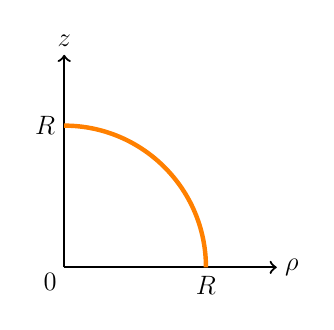
\begin{tikzpicture}[thick, scale=.9, every node/.style={scale=.8}]
	\draw[->] (0,0)--(3,0) node[right] {\large $\rho$};
	\draw[->] (0,0)--(0,3) node[above] {\large $z$};
	\draw[ultra thick, orange] (2,0) node[below, black] {\large $R$} arc (0:90:2) node[left, black] {\large $R$};
	\node at (-0.2,-0.2) {\large 0};
	\end{tikzpicture}
\caption{The minimal surface of a spherical entangling surface in the Poincar{\'e} coordinates of AdS$_{d+1}$.}
\label{fig:Sphere}
\end{figure}

The minimal surface $\gamma_A$ is the solution of the variational problem for the area functional with respect to $z=z(\rho)$,
\begin{align}\label{areaSp}
\CA = L^{d-1} \text{Vol}(\BS^{d-2}) \int_0^R \d\rho\, \frac{\rho^{d-2}}{z^{d-1}(\rho)} \sqrt{1+ (\partial_\rho z)^2} \ .
\end{align}
Solving the equation of motion with the boundary condition $\rho=R$ at the boundary $z=0$,\footnote{The equation of motion is a second-order differential equation, but can be reduced to a first-order one \cite{Bakhmatov:2017ihw,Colgain:2018tzo}.}
the solution turns out to be a hemisphere in any $d$ dimensions \cite{Ryu:2006bv} (see Fig.\,\ref{fig:Sphere})
\begin{align}\label{Sp_sol}
z(\rho) = \sqrt{R^2 - \rho^2} \ .
\end{align}
It follows that the holographic entanglement entropy of a sphere of radius $R$ is
\begin{align}\label{EE_Sphere}
\begin{aligned}
S_A = \frac{L^{d-1}\text{Vol}(\BS^{d-2})}{4G_N} & \int_{\epsilon/R}^1 \d y\, \frac{(1-y^2)^{(d-3)/2}}{y^{d-1}} \ , 
\end{aligned}
\end{align}
where we introduced the UV cutoff $\epsilon \ll 1$ at $z=\epsilon$.

Expanding the integral around $y=0$ and performing the integration near $y=\epsilon /R$, one finds the UV divergent terms consistent with the generic structure in Eq.\,\eqref{EE_Even} for even $d$ and in Eq.\,\eqref{EE_Odd} for odd $d$.
The leading divergent part is proportional to the area of the entangling surface: 
\begin{align}
	\text{Area}(\partial A) = R^{d-2}\,\text{Vol}(\BS^{d-2}) \ ,
\end{align}
which is known to be the area law of entanglement.


\subsubsection{Universal terms}

There is the logarithmic divergence of the entanglement entropy for even $d$, whose coefficient $c_0$ is proportional to the type $A$ anomaly for a spherical entangling surface [see Eq.\,\eqref{Log_EE_C0}],
\begin{align}
	c_0 = (-1)^{d/2+1} A \ .
\end{align}
Compared with Eq.\,\eqref{EE_Sphere}, the type $A$ central charge in a large-$N$ CFT$_d$, described by the Einstein gravity on the AdS$_{d+1}$ spacetime, is determined to be \cite{Myers:2010xs,Myers:2010tj}
\begin{align}
	A = \frac{L^{d-2}}{2G_N} \frac{\pi^{d/2 -1}}{\Gamma (d/2)} \ .
\end{align}

The universal finite term $F$ for odd $d$ in Eq.\,\eqref{EE_Odd} is similarly read off from Eq.\,\eqref{EE_Sphere}.
By analytically continuing $d$ and letting $\epsilon$ be zero before carrying out the integral, we find \cite{Kawano:2014moa}
\begin{align}\label{CFT_F_value}
F = \frac{L^{d-1}}{4G_N} \frac{\pi^{d/2}}{\Gamma(d/2)} \ .
\end{align}
This is always positive thanks to the sign factor put in front of $F$ in Eq.\,\eqref{EE_Odd}.
This universal term is conjectured to decrease monotonically under any renormalization group flow \cite{Myers:2010xs,Myers:2010tj,Klebanov:2011gs}, and known as the holographic $\CC$-theorem \cite{Girardello:1998pd,Freedman:1999gp,Myers:2010xs,Myers:2010tj} that will be discussed in Sec. \ref{ss:RGflow}.


\subsubsection{Relation to thermal entropy on $\BH^{d-1}$}\label{ss:HEE_thermal}
We revisit Eq.\,\eqref{RenyiAndTherm} between the entanglement entropy across a sphere and the thermal entropy on a hyperbolic space derived in Sec. \ref{ss:Rel_to_Therm} from the holographic point of view.
We show, in the hyperbolic coordinates Eq.\,\eqref{AdS_Hyp} of the AdS space, that the minimal surface coincides with the black hole horizon of the AdS topological black hole, and thus the entanglement entropy agrees with the thermal entropy of the black hole.


The Euclidean Poincar{\'e} coordinates Eq.\,\eqref{SpherePoincare} can be mapped by the coordinate transformations
\begin{align}\label{BulkCM}
\begin{aligned}
z &= R\,\frac{1}{r\cosh u + \sqrt{r^2 - 1} \cos \tau} \ , \\
t &= R\, \frac{\sqrt{r^2 -1} \sin(\tau)}{r\cosh u + \sqrt{r^2 -1} \cos \tau} \ , \\
\rho &= R\, \frac{ r \sinh u}{r\cosh u + \sqrt{r^2 -1} \cos \tau} \ ,
\end{aligned}
\end{align}
to the new coordinates 
\begin{align}\label{AdS_Hyp2}
\begin{aligned}
\d s^2 = L^2 \bigg[& \left( r^2 -1\right) \d\tau^2 + \frac{\d r^2}{r^2 -1} \\
	&\qquad + r^2(\d u^2 + \sinh^2 u \,\d\Omega_{d-2}^2)\bigg] \ .
\end{aligned}
\end{align}
This is the Euclidean AdS topological black hole given by Eq.\,\eqref{AdS_Hyp} whose boundary is $\BS^1\times \BH^{d-1}$ (see Fig.\,\ref{fig:TopAdS}).
The $\tau$ coordinate has period $\tau\sim \tau + 1/T$ with the temperature $T=1/(2\pi)$ fixed to avoid the conical singularity at $r=0$.

\begin{figure}[htbp]
\centering
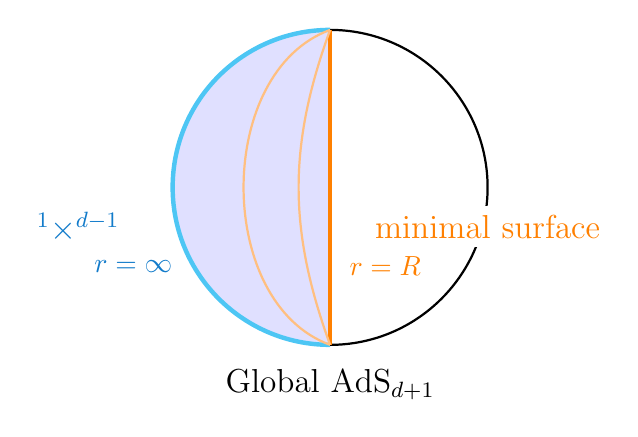
\begin{tikzpicture}[thick]
	\draw[ultra thick, cyan!70, fill=blue!12] (0,2) arc (90:270:2);
	\draw (0,-2) arc (-90:90:2);
	\draw[ultra thick, orange] (0,-2)--(0,2);
	\draw[orange!50] (0,-2) to [out=110, in=250] (0,2);
	\draw[orange!50] (0,-2) to [out=160, in=200] (0,2);
	\node[orange] at (0.7,-1) {$r=R$};
	\node[orange, fill=white] at (2,-0.5) {\large minimal surface};
	\node[cyan!60!blue] at (-2.5,-1) {$r=\infty$};
	\node[cyan!60!blue] at (-3.2,-0.5) {\large $\BS^1 \times \BH^{d-1}$};
	\node[fill=white] at (0,-2.5) {\large Global AdS$_{d+1}$};
\end{tikzpicture}

\caption{The global AdS space obtained by the conformal map Eq.\,\eqref{BulkCM} from the Poincar{\'e} coordinates. The outside of the AdS topological black hole horizon covers half of the global coordinates. The minimal surface (the thick orange curve) in Fig.\,\ref{fig:Sphere} is on the horizon of the AdS topological black hole.
}
\label{fig:TopAdS}
\end{figure}

The entangling surface located at $\rho = R, t=0, z=0$ in the original coordinates Eq.\,\eqref{SpherePoincare} is conformally mapped to a hypersurface at $r=\infty, \tau=0$ and $u=\infty$ in the hyperbolic coordinates Eq.\,\eqref{AdS_Hyp} under the transformations Eq.\,\eqref{BulkCM}.
The minimal surface in the latter coordinates anchored on constant time $\tau=0$ and $r=\infty, u=\infty$ is obtained by extremizing the area functional with respect to $r=r(u)$,
\begin{align}
\begin{aligned}
\CA = L^{d-1} \int_0^\infty \d u\, (r \sinh u)^{d-2} \sqrt{r^2 + \frac{(\partial_u r)^2}{r^2 -1}} \ .
\end{aligned}
\end{align}
It is easy to check $r=1$ is the solution to the equation of motion, which
is nothing but the horizon of the topological AdS black hole.
We thus find the holographic entanglement entropy is equal to the black hole entropy \cite{Casini:2011kv},
\begin{align}
S_A(R) = S_\text{BH}(T) = S_\text{therm}(T)\ ,
\end{align}
where we used one more relation between the AdS$_{d+1}$ black hole entropy $S_\text{BH}$ and the thermal entropy $S_\text{therm}$ of the dual CFT$_d$ on $\BH^{d-1}$ at temperature $T$.
This completes the holographic derivation of Eq.\,\eqref{RenyiAndTherm}.


\subsection{Holographic R{\'e}nyi entropy}\label{ss:HRE}
Before concluding this section, we make a few comments on the holographic calculation of the R{\'e}nyi entropy.
We first derive the holographic formula of the modular entropy in a similar manner to the holographic entanglement entropy in Sec. \ref{ss:HEE} and show it is given by the area of a cosmic brane.
The R{\'e}nyi entropy is constructed out of the modular entropy by Eq.\,\eqref{Renyi_Modular}.
As an example, we calculate the holographic R{\'e}nyi entropy across a spherical entangling surface in CFT .


\subsubsection{A derivation of the holographic formula}
The argument for deriving the Ryu-Takayanagi formula in Sec. \ref{ss:HEE_Derivation} has more implications for the holographic description of quantum entanglement than it appears.
The modular entropy Eq.\,\eqref{ModularEntropy} written in terms of the partition function
\begin{align}
	\tilde S_n &= (1 - n\partial_n) (\log Z_n - n\log Z)
\end{align}
can be turned, with the GKP-W relation and the bulk-per-replica action Eq.\,\eqref{Bulk_Per_Replica}, into
\begin{align}
	\begin{aligned}
		\tilde S_n 
		&= (n\partial_n -1 ) \left[ n (\hat I [\hat \CB_n ] - I_\text{bulk} [ \CB ] )\right] \  , \\
		&=  n^2 \partial_n \hat I [\hat \CB_n] \ .
	\end{aligned}
\end{align}
This reminds us of the holographic definition of entanglement entropy Eq.\,\eqref{ARE_II}, and one can recycle the resulting relation \eqref{BPR_action_Der} to find \emph{the holographic formula of the modular entropy} \cite{Dong:2016fnf},
\begin{align}\label{HRE_formula}
	\tilde S_n = \frac{\CA_n}{4G_N}\bigg|_{\delta \hat I = 0, \,\partial \gamma^{(n)}_A = \Sigma} \ .
\end{align}
It resembles the Ryu-Takayanagi formula \eqref{ARE} and actually reproduces it when $n=1$.
This formula, however, contains the area of a codimension-two \emph{cosmic brane} $\gamma_A^{(n)}$ with tension $\delta_n/(8\pi G_N)$ that backreacts to the bulk geometry.
Hence it is more intricate in practice than the case of the Ryu-Takayanagi formula \eqref{ARE} as we have to fix the location of the cosmic brane by solving the equations of motion of the action $\hat I$ describing the Einstein gravity coupled to the cosmic brane and possibly matter fields as indicated by the subscript $\delta \hat I = 0$ in Eq.\,\eqref{HRE_formula} [see Eq.\,\eqref{BPR_action_Der} for the definition of $\hat I$].
We are also able to build the \emph{holographic R{\'e}nyi entropy} by combining Eq.\,\eqref{HRE_formula} with the relation \eqref{Renyi_Modular}.

Given the holographic formula of the R{\'e}nyi entropy, one may ask whether it satisfies the inequalities Eqs.\,\eqref{RenyiIneq1}-\eqref{RenyiIneq4} characterizing the R{\'e}nyi entropy.
To this end it is enough to check the three inequalities Eq.\,\eqref{Modular_Ineq} implying the non-negativities of the modular energy, entropy and capacity.
The easiest one to show is the inequality $\tilde S_n \ge 0$ that follows from the non-negativity of the area of a cosmic brane in Eq.\,\eqref{HRE_formula}.
The non-negativity of the modular energy $E\ge 0$ becomes clear by expressing $E$ in the form
\begin{align}
	E  = I_\text{bulk}[\hat \CB_n] - I_\text{bulk}[\CB] + \frac{\CA_n}{4G_N} \ ,
\end{align}
and invoking $\CB$ the on-shell solution with the least action while $\hat \CB_n$ is not necessarily so.
The last inequality $C\ge 0$ for the modular capacity is most nontrivial and turns out to require the stability of the bulk geometry $\CB_n$ \cite{Nakaguchi:2016zqi}.
It remains an open issue whether and when such a stability condition is guaranteed to hold in the holographic setup.


\subsubsection{Spherical entangling surface in CFT}

We have seen in Sec. \ref{ss:HEE_thermal} that the entanglement entropy across a spherical entangling surface in CFT is equal to the thermal entropy on $\BH^{d-1}$ at inverse temperature $2\pi R$ and can be calculated holographically as the black hole entropy in the dual AdS spacetime.
Here we see the holographic formula of the modular entropy \eqref{HRE_formula} also has an elegant interpretation as a black hole entropy when the entangling surface is spherical in accordance with the CFT story in Sec. \ref{ss:Renyi_CFT} \cite{Hung:2011nu}.

The AdS topological black hole given by Eq.\,\eqref{AdS_Hyp2} is a particular case of the following AdS black hole,
\begin{align}\label{AdS_Hyp_Renyi}
\d s^2 = L^2\left[ f(r)\, \d\tau^2 + \frac{\d r^2}{f(r)}+ r^2(\d u^2 + \sinh^2 u \,\d\Omega_{d-2}^2)\right] \ ,
\end{align}
where the function $f(r)$ vanishes at $r = r_H$,
\begin{align}
	f(r) =  r^2 -1 - \frac{r_H^{d-2}}{r^{d-2}}\left( r_H^2 - 1\right) \ .
\end{align}
This black hole has a temperature parametrized by $r_H$,
\begin{align}\label{RenyiBHTemp}
	T(r_H) = \frac{1}{4\pi} \left[ d\, r_H - \frac{d-2}{r_H} \right] \ ,
\end{align}
and the dual CFT lives on the boundary that is a hyperbolic space $\BH^{d-1}$ at finite temperature $T(r_H)$.

In this setup, the codimension-two cosmic brane in \eqref{HRE_formula} is at the black hole horizon and the modular entropy can be identified with the thermal entropy by matching the black hole temperature Eq.\,\eqref{RenyiBHTemp} with $T_n = 1/(2\pi n)$.
By setting $r_H$ to
\begin{align}
	r_n = \frac{1+\sqrt{d\,n^2(d - 2) + 1}}{d\, n} \ ,
\end{align}
the black hole entropy at temperature $T_n$ becomes 
\begin{align}
	\tilde S_n = S_\text{therm}\left(T_n\right) = \frac{\text{Vol}(\BH^{d-1})L^{d-1}}{4G_N} r_n^{d-1} \ .
\end{align}
Performing the integration in Eq.\,\eqref{Renyi_Modular} or Eq.\,\eqref{RenyiTherm} leads to the R{\'e}nyi entropy,
\begin{align}
\begin{aligned}
	S_n 	&= \frac{\text{Vol}(\BH^{d-1})L^{d-1}}{4G_N}\frac{n}{2(n-1)}\left(2 - r_n^{d-2} - r_n^d\right) \ .
\end{aligned}
\end{align}



\endinput